%---------------------------------------------------------------------------------
%--------------------------Set the variables for every client---------------------
%---------------------------------------------------------------------------------
\renewcommand{\hostname}{Example}
\renewcommand{\os}{Linux OS Soft XP}
\renewcommand{\ip}{42.42.42.42}
\renewcommand{\tcpports}{1,2,3}
\renewcommand{\udpports}{23,42}
\renewcommand{\vuln}{CVE-123-42 \glqq Stupid Idiot User\grqq}
\renewcommand{\vulnx}{CVE-123-43 \glqq Very Stupid Idiot User Again\grqq} 
%%%Did you get root? Comment out if you only got low priv access
\def\root{}   %%% Define root if you got root shell


%----------------------------------------------------------------------------------
%-------------------------------Auto generated content-----------------------------
%----------------------------------------------------------------------------------

\section{\hostname}
\subsection{Service Enumeration}

\begin{table}[h]
	\begin{tabular}{|c|c|}
		\hline
		\multicolumn{2}{|c|}{\textbf{\hostname}}\\\hline\hline
		Type         & Open ports   \\\hline
		TCP          & \tcpports{}  \\\hline
		UDP          & \udpports{}  \\\hline\hline
		\textbf{\os} & \textbf{\ip} \\\hline
	\end{tabular}
	\caption{Service enumeration \hostname}
\end{table}

\subsection{Remote Access Exploitation}

\paragraph{Vulnerability Exploited:}
\vuln

%----------------------------------------------------------------------------------
%-------------------------------Start writing here---------------------------------
%----------------------------------------------------------------------------------
 
\paragraph{Vulnerability Explanation:}
BLA BLA WRITE SOMETHING HERE BLA BLA WRITE SOMETHING HERE BLA BLA WRITE SOMETHING HERE BLA BLA WRITE SOMETHING HERE BLA BLA WRITE SOMETHING HERE BLA BLA WRITE SOMETHING HERE BLA BLA WRITE SOMETHING HERE BLA BLA WRITE SOMETHING HERE BLA BLA WRITE SOMETHING HERE BLA BLA WRITE SOMETHING HERE BLA BLA WRITE SOMETHING HERE BLA 

\paragraph{Severity:}
\textbf{\textcolor{red}{Critical}}

\paragraph{Proof of Concept:} 
Modifications to the existing exploit was needed and is highlighted in red.
\begin{lstlisting}[caption={Exploitation of \hostname}]
SELECT * FROM login WHERE id = **@1 or 1=1@** AND user LIKE "\%root\%"
In the code section :
*@Green Text@*
**@Red Text@**
***@Blue Text@***
\end{lstlisting}

\paragraph{Screenshot:} 
\begin{figure}[H]
	\centering
	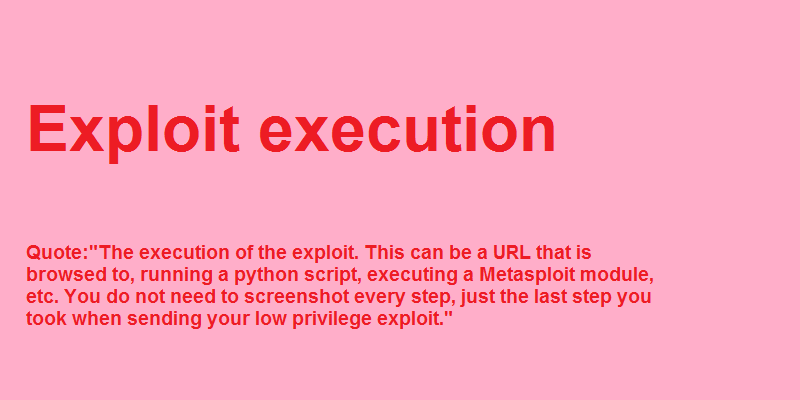
\includegraphics [width=1.0\textwidth]{./hosts/\hostname/exploitexecution.png}
	%scale 0.5 bedeutet 50% der originalgröße
	%angle=90 Grafik um 90° drehen
	\caption[Exploitation of \hostname]{Exploitation of \hostname}
\end{figure}

\paragraph{Proof:} %Print proof for local exploit here
\begin{lstlisting}[caption={Proof of local shell on \hostname}]
hostname && id && ifconfig && cat local.txt
\end{lstlisting}
\begin{figure}[H]
	\centering
	
\includegraphics [width=\textwidth]{./hosts/\hostname/local.png}
	\caption[Local shell of \hostname]{Local shell of \hostname}
\end{figure}

%----------------------------------------------------------------------------------
%------------------------------Conditional Privilege Escalation Block--------------
%----------------------------------------------------------------------------------
\ifdefined\root

%----------------------------------------------------------------------------------
%------------------------------Part for Priv escalation----------------------------
%----------------------------------------------------------------------------------
\subsection{Privilege Escalation}

\paragraph{Vulnerability Exploited:}
\vulnx

\paragraph{Vulnerability Explanation:}
BLA BLA WRITE SOMETHING HERE BLA BLA WRITE SOMETHING HERE BLA BLA WRITE SOMETHING HERE BLA BLA WRITE SOMETHING HERE BLA BLA WRITE SOMETHING HERE BLA BLA WRITE SOMETHING HERE BLA BLA WRITE SOMETHING HERE BLA BLA WRITE SOMETHING HERE BLA BLA WRITE SOMETHING HERE BLA BLA WRITE SOMETHING HERE BLA BLA WRITE SOMETHING HERE BLA 

\paragraph{Severity:}
\textbf{\textcolor{red}{Critical}}

\paragraph{Proof of Concept:} 
Modifications to the existing exploit was needed and is highlighted in red.
\begin{lstlisting}[caption={Exploitation of \hostname}]
SELECT * FROM login WHERE id = **@1 or 1=1@** AND user LIKE "\%root\%"
In the code section :
*@Green Text@*
**@Red Text@**
***@Blue Text@***
\end{lstlisting}

\paragraph{Screenshot:} 
\begin{figure}[H]
	\centering
	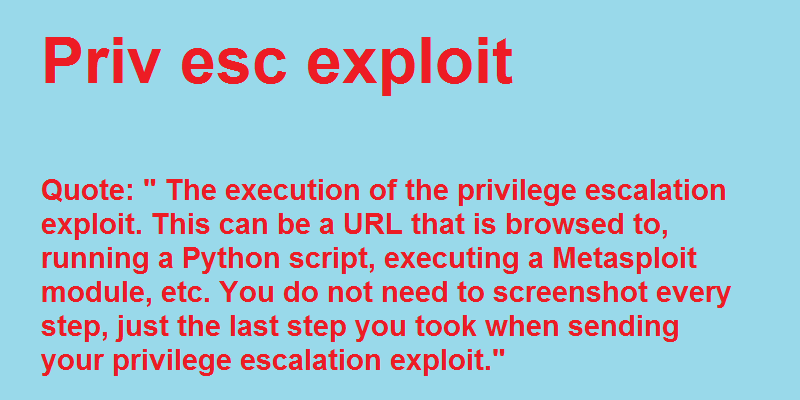
\includegraphics [width=1.0\textwidth]{./hosts/\hostname/privescexploit.png}
	\caption{Priv escalation exploit of \hostname}
\end{figure}

\paragraph{Proof:}
\begin{lstlisting}[caption={Post exploitation of \hostname}]
hostname && id && ifconfig && cat proof.txt
\end{lstlisting}

\begin{figure}[H]
	\centering
	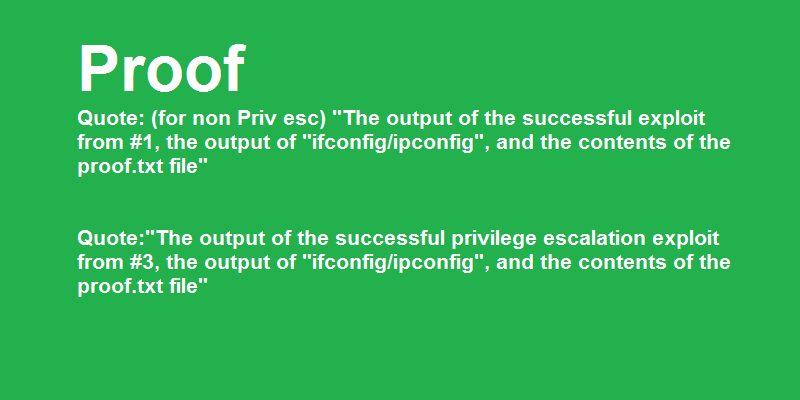
\includegraphics [width=\textwidth]{./hosts/\hostname/proof.png}
	\caption[Proof of \hostname]{Proof of \hostname}
\end{figure}
\fi % End of if-block
%----------------------------------------------------------------------------------
%--------------------------------------End of Priv Esc Block-----------------------
%----------------------------------------------------------------------------------


